\chapter{Metodologia dell’analisi}

\section{Selezione degli eventi analizzati}
Per analizzare come il linguaggio giornalistico possa essere influenzato dalla politica, il nostro gruppo ha scelto sei momenti significativi legati ad attività pubbliche e politiche del neo eletto presidente degli Stati Uniti d'America Donald Trump tra il 2024 e il 2025.\\
Si tratta di eventi estremamente differenti tra loro, dal comizio elettorale di Indianola, in Iowa, al World Economic Forum di Davos, tutti però accomunati da una forte visibilità, sia a livello nazionale che internazionale. \\
La scelta è ricaduta su questi episodi non solo per la loro posizione temporale, ma anche per la varietà dei temi trattati: immigrazione, politica energetica, sicurezza nazionale, economia e relazioni internazionali. \\
Ogni discorso ci ha offerto uno spunto utile per comprendere come il modo di raccontare i fatti possa cambiare a seconda della linea editoriale del giornale. \\
È necessario sottolineare che i discorsi analizzati sono stati tenuti in fasi cruciali del percorso politico di Trump: durante le primarie, l’accettazione della candidatura, successivo alla vittoria elettorale, all’insediamento ed infine in un importante evento internazionale durante il quale ha rilanciato la sua agenda. \\
Questa varietà, sia nei tempi sia nei contenuti, ci ha permesso di raccogliere un campione estremamente ampio e necessario per evidenziare tendenze ricorrenti e differenze di stile tra le varie aree ideologiche del panorama dell’informazione.\\

\section{Criteri di classificazione delle fonti (progressiste, neutrali, conservatrici)}
Dividere le testate giornalistiche in tre categorie, progressiste, neutrali e conservatrici, è stato un passaggio fondamentale nell’analisi, tale distinzione si è basata in primis su una ricerca delle posizioni editoriali storiche delle testate considerate, valutando sia l’orientamento dichiarato sia quello che si può intuire dal linguaggio e dello stile nel tempo. \\
Per rendere la nostra classificazione più oggettiva, abbiamo analizzato anche articoli specifici, concentrandoci su parole usate, tono e scelta delle informazioni.\\
Le testate progressiste si distinguono per un linguaggio critico ed a volte allarmante, che mette in evidenza presunte tendenze autoritarie, sessiste o razziste nei discorsi di Trump. Le testate conservatrici, al contrario, tendono a descrivere Trump come un leader carismatico, simbolo di rinascita nazionale e garante della sicurezza attraverso un linguaggio spesso enfatico, patriottico che punta a creare un legame emotivo con il lettore. Le fonti neutre, pur essendo poche, offrono un buon termine di confronto: usano un tono descrittivo, riportando fatti e dati senza giudizi evidenti. Tuttavia, anche in questi casi è complesso parlare di "vera" neutralità, in quanto la scelta delle informazioni, delle immagini e dell’impostazione dell’articolo può mostrare una certa direzione narrativa.

\section{Metriche di analisi (numero articoli, sentiment analysis, parole chiave)}
Per questa analisi ci siamo basati su tre strumenti principali, combinando approcci sia quantitativi che qualitativi. Il primo è stato il conteggio degli articoli usciti per ogni evento, pubblicati da testate con orientamenti politici diversi: questo ci ha aiutato a capire quanto spazio ciascun evento ha ricevuto e se ci sono state differenze nel modo in cui è stato raccontato. Il secondo strumento è la sentiment analysis, che usa algoritmi per assegnare un valore emotivo(positivo, negativo o neutro) alle parole presenti nei testi. In questo modo è stato possibile vedere come lo stesso fatto venga presentato in modi anche molto diversi, a seconda del linguaggio usato: ad esempio, un giornale conservatore può parlare di “epoca d’oro per l’America”, mentre uno progressista può usare termini come “dittatura capitalistica”. Il terzo strumento ha riguardato l’analisi delle parole chiave, che serve a individuare i termini più frequenti nei vari articoli e capire che significato politico o ideologico possono avere. In totale, queste analisi sono state applicate a oltre ottanta articoli, permettendoci di fare un confronto abbastanza dettagliato. Da tutto questo è emersa una tendenza piuttosto chiara: il linguaggio è spesso polarizzato, con strategie retoriche usate apposta per rafforzare una certa visione politica o sociale. In pratica, il giornalismo non si limita a raccontare i fatti, ma contribuisce anche a costruire un’idea precisa della realtà.

\begin{figure}[H]
    \centering
    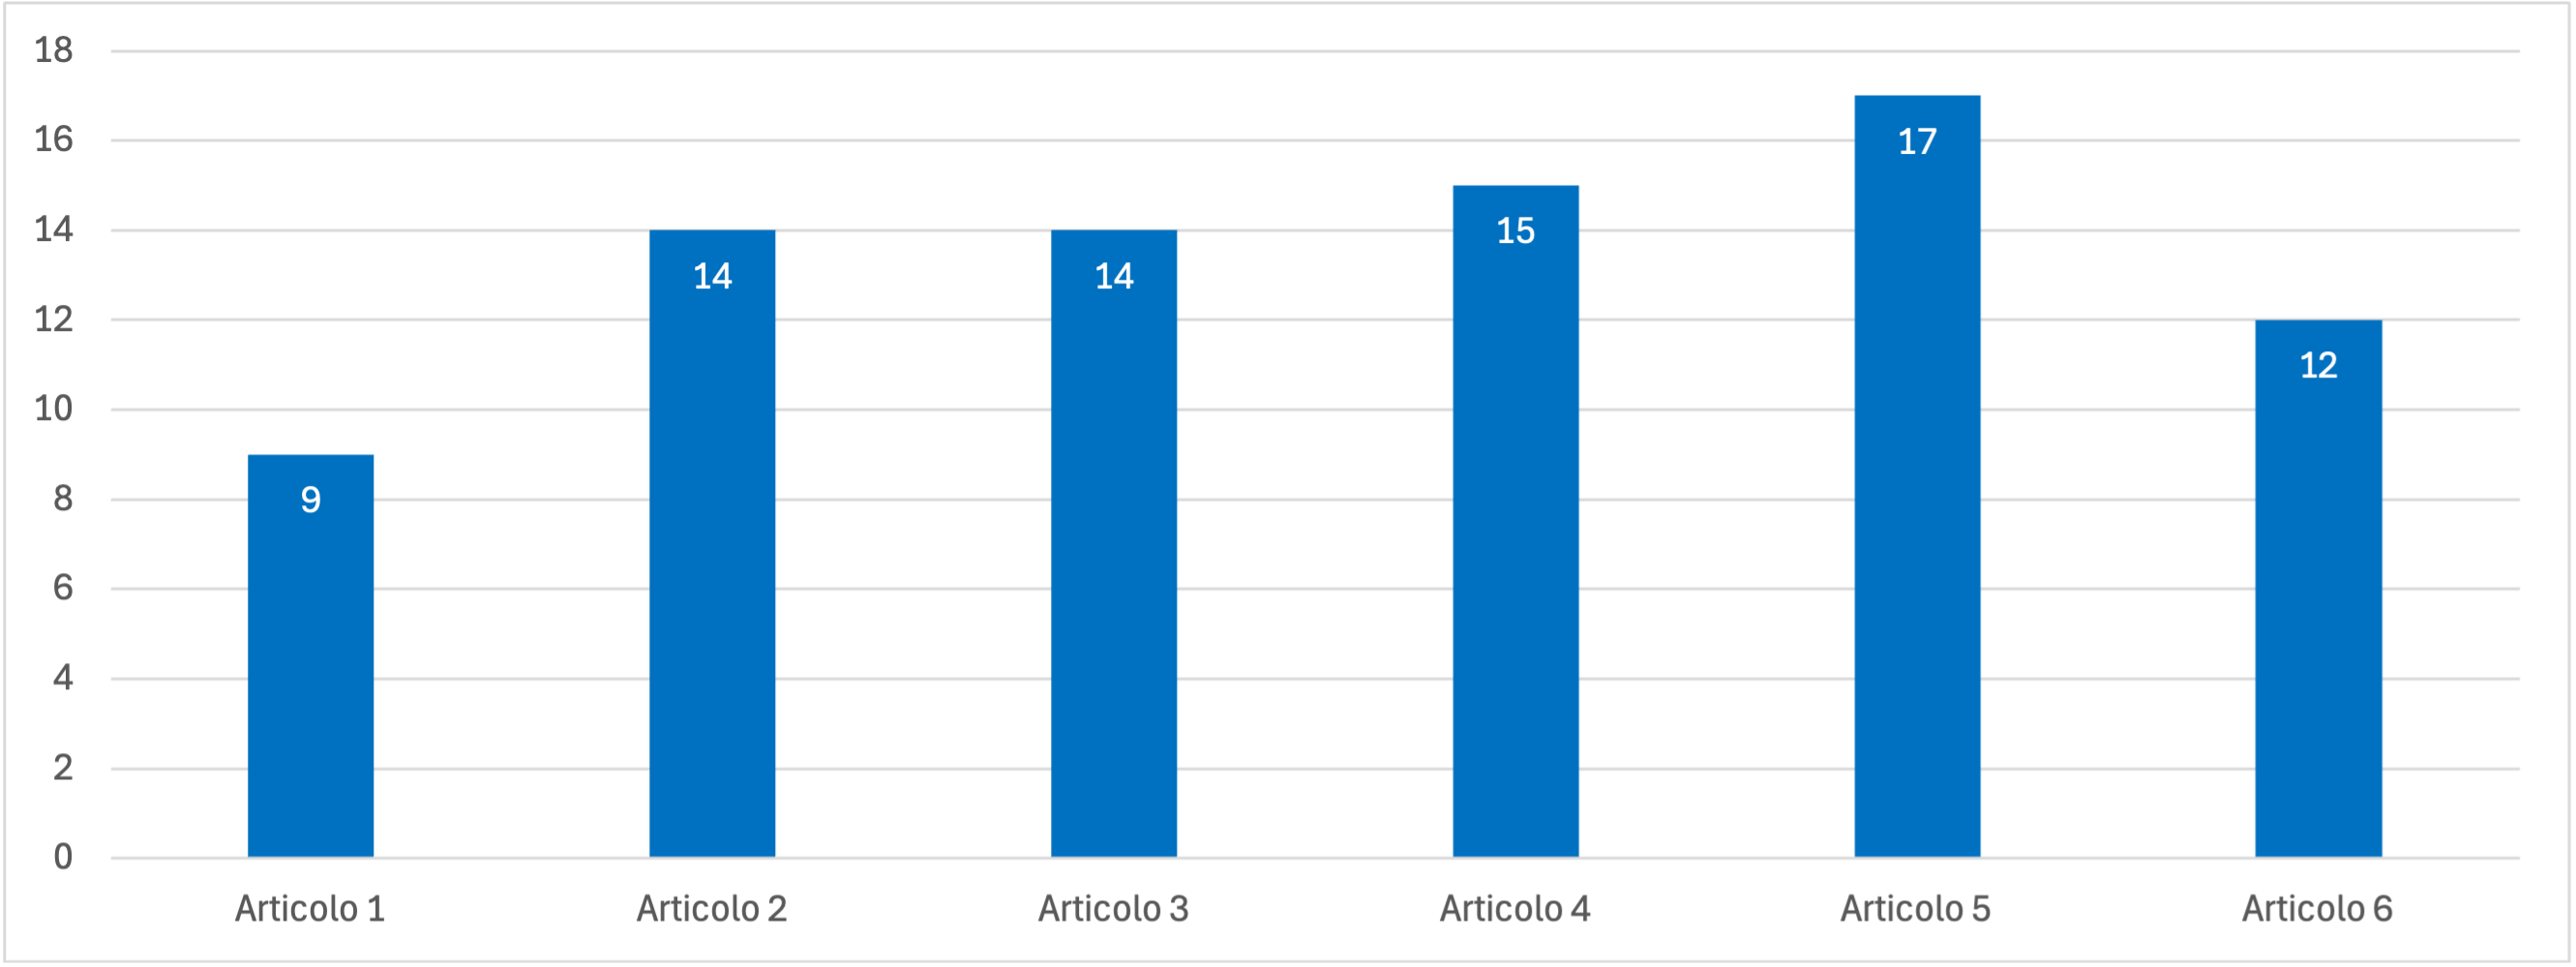
\includegraphics[width=1\linewidth]{Immagini/Istogramma Articoli.png}
    \caption{Istogramma articoli.}
    \label{fig:istogramma-articoli}
\end{figure}